\documentclass{article}
\usepackage[utf8]{inputenc}
\usepackage{geometry}
\usepackage{graphicx}
\usepackage{listings}

\usepackage{amsfonts}
\newcommand{\Z}{\mathbb{Z}}

\def\code#1{\texttt{#1}}
\newcommand\tab[1][0.5cm]{\hspace*{#1}}

\geometry{a4paper, margin=0.7in}

\title{Trabajo Practico 2}
\author{De Rosa - Schapira - Guerrero}
\date{Primer Cuatrimestre 2017}

\begin{document}
    \pagenumbering{gobble}
    \maketitle
    \newpage
    \pagenumbering{roman}
    \tableofcontents
    \newpage
    \pagenumbering{arabic}

    \section{Clases de complejidad}
    \tab A continuación se resolverán los seis problemas planteados, en caso de ser polinomiales se propondrá un
    pseudo-código del algoritmo que lo resuelva y en caso de ser NP-Completos se hará la reducción correspondiente.
    \begin{enumerate}
        \item \textbf{Se tiene un conjunto de n actividades para seleccionar. Cada actividad tiene asociados un tiempo de
            inicio y tiempo de fin. Se dice que un conjunto de actividades es compatible si no hay dos que se
            superpongan en un tiempo. Se pide un algoritmo que devuelva verdadero o falso de acuerdo a si se
            puede encontrar un subconjunto compatible de tamaño k o superior.} %\\
            \tab Este problema pertenece a $P$, pues puede ser resuelto de la siguiente manera: %\\
            \begin{lstlisting}
Funcion seleccionar_actividades ( ListaAct )
    actTiempoFin = ordenar segun tiempos de fin ( ListaAct )

    k = 0
    #se agarran todas las actividades menos la primera y la ultima
    for i in xrange(1,  len(ListaAct)-1 ):
    si la actTiempoFin[ i ].inicio > actTiempoFin[ k ].fin:
        k=i
    else:
        return false

    return true
            \end{lstlisting}

            \tab El algoritmo ordena las actividades en base al tiempo de finalización y luego se recorren $n-2$
            actividades verificando la compatibilidad.
            \tab Para que este algoritmo funcione en tiempo polinomial la lista de actividades debe ordenarse
            de manera eficiente. Por ejemplo, utilizando MergeSort que es, en su peor caso $O(n Log(n))$, siendo
            $n$ la cantidad de elementos.
            \tab Suponiendo que esto sea así, el ordenamiento será $O(n Log(n))$ y el ciclo subsiguiente $O(n)$,
            resultando el algoritmo $O(n Log(n))$ y, por lo tanto, perteneciente a $P$.

        \item \textbf{Se tiene un conjunto de n actividades para seleccionar. Cada actividad tiene asociados un conjunto de
            tiempos de inicio y fin. Se dice que un conjunto de actividades es compatible si no hay dos que se
            superpongan en un tiempo. Se pide un algoritmo que devuelva verdadero o falso de acuerdo a si se
            puede encontrar un subconjunto compatible de tamaño k o superior.} %\\

            \tab Este problema pertenece a la familia de los $NP-C$ y esto se puede demostrar haciendo una reducción
            del problema de \emph{k-Coloreo} de un Grafo (que llamaremos $K$), que es $NP-C$. Haciendo esto,
            demostraremos que nuestro problema ($P$) verifica $K \leq_{P} P$.

            \tab\tab Supongamos que tenemos el grafo $G$:
            %\begin{center}
            %    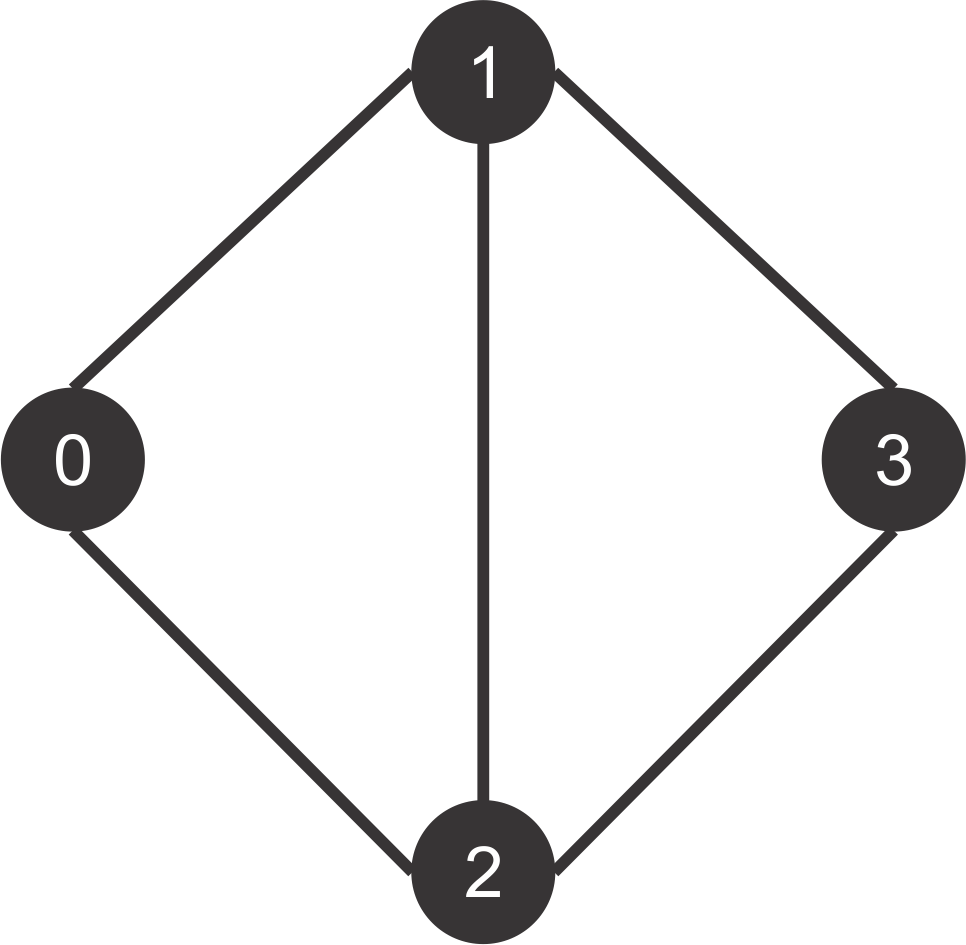
\includegraphics[width=9cm, height=5cm]{images/Problema2}
            %\end{center}
                \tab A partir de las incidencias de cada vértice $v_{i}$, es decir, sabiendo a que otros vertices $v_{j}$
                es adyacente cada $v_{i}$ podemos saber qué vértices no deben repetir colores. \\
                \tab Sabiendo esto, se puede generar un diccionario donde se guarda la información sobre que conjuntos
                de vértices compartiran un intervalo con inicio $i_{k}$ y fin $f_{k}$, pues esos serán los vértices que no
                serán compatibles. El diccionario tendría la forma
                    $\{ [0, 1, 2] : [i_{0}, f_{0}], [1, 3] : [i_{1}, f_{1}], [2, 3] : [i_{2}, f_{2}] \}$
                y se iría completando avanzando por el grafo y, para cada $v_{i}$, verificando si ya comparte un conjunto con
                todos sus vecinos y en caso contrario, creando uno nuevo, con un nuevo intervalo. \\
                \tab Una vez generado el diccionario, se procedería a identificar a cada $v_{i}$ como una actividad $a_{i}$
                con los intervalos correspondientes. Esto resultaría en:
                    $\{ 0 : [[i_{0}, f_{0}]], 1 : [[i_{0}, f_{0}], [i_{1}, f_{1}]], 2 : [[i_{0}, f_{0}], [i_{2}, f_{2}]],
                    3 : [[i_{1}, f_{1}], [i_{2}, f_{2}]] \}$ \\
                \tab Finalmente, y con cada vértice adaptado al modelo de actividades del problema original, podríamos
                resolver el problema $K$ procesando nuestras nuevas actividades con el algoritmo
                que resuelva el problema $P$ original, para un $k$ cualquiera. \\
                \tab Por lo tanto, $K \leq_{P} P$ y, entonces, $P \in NP-C$.

        \item \textbf{En teoría de grafos, un camino hamiltoniano es un camino que visita cada vértice del grafo exactamente
            una vez. Se pide un algoritmo que indique si un grafo G tiene un camino hamiltoniano o no.} %\\

            %TODO

        \item \textbf{En teoría de grafos, un camino hamiltoniano es un camino que visita cada vértice del grafo exactamente
            una vez. Se pide un algoritmo que indique si un digrafo acíclico D tiene un camino hamiltoniano o no.} %\\

            \tab Dado que a todo Grafo Dirigido Acíclico (\emph{DAG}) se le puede hacer un ordenamiento topológico tal que los
            vértices queden ordenados como $(v_{1}, v_{2})(v_{2},v_{3})...(v_{n-1}, v_{n})$ se ordena el grafo $G$ de tal manera.
            Una vez logrado esto, se recorren todos los vértices verificando que haya una arista desde cada $v_{i}$ a cada $v_{j}$,
            con $i < j$. Pues, dado que en el camino Hamiltoniano no se puede volver atrás, la única manera de recorrer todos los vertices
            es no salteandose ninguno. \\
            \tab A continuación se muestran los algoritmos para el ordenamiento topológico de un \emph{DAG} y la solución
            al problema planteado:
            \begin{lstlisting}
funcion ordenTopologico(G):
    L = Lista vacia que contendra los elementos orenados
    S = Set con todos los vertices sin aristas entrantes
    while S no esta vacia:
        tomar un vertice v de S
        L.append(v)
        para cada vertice u con una arista(v, u):
            scar la arista(v, u) de G
            si u no tiene mas aristas entrantes:
                S.add(u)
    si G tiene aristas:
        return error (G tiene al menos un ciclo)
    else
        return L

funcion tieneCaminoHamiltoniano(G):
    #Primero se ordena a los vertices con un orden topologico (O(V+E))
    L = ordenTopologico(G)
    #Luego se verifica que exista una arista de cada vertice al siguiente (O(V))
    for i=0...len(L)-2:
        if ( no hay arista(L[i], L[i+1]) ):
            return False
    return True
            \end{lstlisting}
            \tab Dado que el ordenamiento topólogico es $O(|V| + |E|)$ y el ciclo de verificación es $O(|V|)$
            el algoritmo es polinómico y tiene un tiempo asintótico de $O(|V|+|E|)$.


        \item \textbf{Se tiene un grafo dirigido y pesado G, cuyas aristas tienen pesos que pueden ser negativos. Se pide
            devolver verdadero o falso de acuerdo a si el grafo tiene algún ciclo con peso negativo.} \\
            \tab El problema propuesto puede ser resuelto utilizando el algoritmo de Bellman-Ford (descripto en la segunda
            parte de este trabajo) en tiempo polinómico, pues el algoritmo es $O(|V||E|)$ siendo $|V|$ la cantidad de
            vertices y $|E|$ la cantidad de aristas, el cual, en el peor de los casos será $|E|=|V|^2$ por lo que
            el algoritmo tendrá un orden $O(n^3)$ con $n = |V|$. El algoritmo es el siguiente:
            \begin{lstlisting}
BellmanFord(Grafo, verticeInicial):
    # se definen incialmente todas las distancias en INFINITO
    # menos la del verticeInicial que se define en 0
    for vertice in Grafo:
        distancias[vertice] = INFINITO
        padres[vertice] = None
    distancia[verticeInicial] = 0
    #se relajan todas las aristas
    for i=0...len(Grafo):
        #Se itera para todos los vertices del grafo
        for each arista(u, v) in aristas:
        if distancias[v] > distancias[u] + peso(u, v):
              distancias[v] = distancias[u] + W(u, v)
              padres[v] = u
    #se verifica si hay ciclos negativo
    for each arista(u, v) in aristas:
        if distancia[v] > distancia[u] + peso(u, v):
            #Hay ciclo negativo
            return True
        return False
            \end{lstlisting}

        \item \textbf{Se tiene un grafo dirigido y pesado G, cuyas aristas tienen pesos que pueden ser negativos. Se pide
            devolver verdadero o falso de acuerdo a si el grafo tiene algún ciclo con exactamente igual a cero.} \\
            \tab Este problema es $NP-C$ y lo demostraremos reduciéndo el \emph{Subset Sum Problem (S)} a nuestro
            problema, que llamaremos $Z$. Demostrando así que $S \leq_{P} Z$. \\
            \tab\tab Supongamos que tenemos un problema $S$ con una entrada $W = \{w_{1}, ..., w_{n}\} \subseteq \Z$
                la cual es aceptada por $S$ si existe un $A\subseteq \Z$ tal que: $$\sum_{a \in A} a = 0$$.
                \tab Lo que haremos es resolver el problema S a través del problema propuesto. Para esto,
                construiremos un grafo $G = (V, E)$ con $2n$ vertices de la siguiente manera:
                \begin{itemize}
                    \item Para cada elemento $w_{i}$ creamos dos vertices: $u_{i}$ y $v_{i}$.
                    \item Para cada $v_{i}$ agregamos la arista $(v_{i}, u_{i})$ a $E$ con peso $w_{i}$.
                    \item Para cada $u_{i}$ y cada $v_{j}$ agregamos la arista $(u_{i}, v{j})$ a $E$ con peso $0$.
                \end{itemize}
            \tab\tab Por lo tanto, un problema $S$ de tres elementos formaría un grafo de la siguiente forma:
                \begin{center}
                    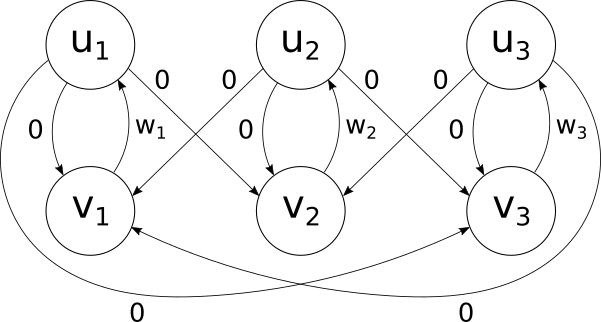
\includegraphics[width=9cm, height=5cm]{images/Problema6}
                \end{center}
            \tab\tab Una vez que tenemos esto planteado, envíamos nuestro grafo a un hipotético algoritmo
                que resuelva el problema $Z$ teniendo en cuenta que:
                \begin{itemize}
                    \item Si hay un ciclo, pasa por al menos un elemento completo (esto es, $u_{i}$ y $v_{i}$).
                    \item Al pasar por dicho elemento, la distancia total aumenta en $w_{i}$ (pues los pesos son $0$
                    y $w_{i}$).
                    \item Si un ciclo pasa por múltiples elementos, la distancia total será la suma de todos sus pesos.
                \end{itemize}
            \tab\tab Dicho esto, si el algoritmo que resuelve $Z$ encuentra un ciclo de distancia $0$, entonces existe
            un subconjunto de $W$ que suma $0$. Por lo tanto $S \leq_{P} Z$ y entonces $Z \in NP-C$.


    \end{enumerate}

    \newpage

    \section{Algoritmos de camino mínimo}
        \subsection{Comparación de algoritmos}
            \tab Todos los algoritmos se basan en una operación llamada \emph{relajación de aristas}. Relajar
        la arista \code{v->w} significa verificar si la mejor manera de ir de \code{s} a \code{w} es \code{s->v->w}
        y, en tal caso, actualizar la información contenida en \code{distancia[w]} y \code{padre[w]}.

            \subsubsection{Dijkstra}
            \tab Este algoritmo encuentra el camino mínimo desde un vértice en particular hacia todo
            el resto de los vertices (\emph{single-source shortest-path problem}). \\
            \tab Es un algoritmo Greedy y se basa en tomar siempre, entre todos los vértices adyacentes,
            el que esté más cerca del origen y ver si se puede llegar más rápido a través de este vértice a los demás
            actualizando las distancias a cada paso hasta que el vértice no utilizado más cercano sea el destino. \\
            \tab Es el más veloz de los tres algoritmos implementados con un tiempo asintótico de
            $O(|E|Log(|V|))$ pero los pesos de las aristas deben ser \emph{siempre} $W >= 0$, en otro caso, falla.

            \subsubsection{Floyd-Warshall}
            \tab Este algoritmo resuelve el \emph{all-pairs shortest path problem}, es decir, hallar los
            caminos mínimos entre todos los pares de vértices del grafo. \\
            \tab Utiliza la técnica de la Programación Dinámica y se basa en que cada iteracion se mejora
            el camino minimo entre dos vertices, hasta llegar al menor de todos. Este algoritmo trabaja
            directamente con la matriz de adyacencia del grafo y para cada $v_{i}$, busca el camino
            mínimo hasta la $v_{j}$ suponiendo que solo se puede pasar por $\{ v_{0}, ..., v_{k-1}\}$.\\
            \tab Tiene un tiempo asintótico de $O(|V|^3)$ pero si bien es el más lento de los tres
            algoritmos analizados permite, una vez que se ejecuta, adquirir el camino mínimo entre cualquier
            par de vértices del grafo en $O(1)$. Además, si bien se supone que el grafo no tiene ciclos negativos,
            se puede utilizar el algoritmo para detectarlos analizando la diagonal de la matriz de camino.

            \subsubsection{Bellman-Ford}
            \tab Utiliza la técnica de la Programación Dinámica para resolver el \emph{single-source shortest-path problem}.
            \tab El algoritmo se basa en repetir $|V| - 1$ veces el proceso de relajación de aristas para
            las $|E|$ aristas del grafo. Una vez realizado esto, se relajan la|s $|E|$ aristas una vez mas.
            Si se obtiene un mejor resultado que antes, entonces el grafo tiene ciclos negativos. \\
            \tab El tiempo asintótico de este algoritmo es, entonces, $O(|V||E|)$, que es más lento que Dijkstra
            pero permite detectar ciclos negativos.

            \subsubsection{Conclusiones}
            \tab Concluyendo esta sección, podemos decir que:
            \begin{itemize}
                \item Dijkstra es la mejor opción para resolver el \emph{single-source shortest-path problem}
                cuando sabemos que no habrá ciclos negativos y todas las aristas tienen peso positivo.
                \item Bellman-Ford es la mejor opción cuando queremos detectar ciclos negativos o tenemos un
                grafo con aristas de peso negativo.
                \item Floyd-Warshall es la mejor opción cuando queremos resolver el \emph{all-pairs shortest path problem}
                y además permite hallar ciclos negativos.
            \end{itemize}
            \tab En cuanto a la relación de tiempos de ejecución, aquí hay un gráfico descriptivo:
            \begin{center}
                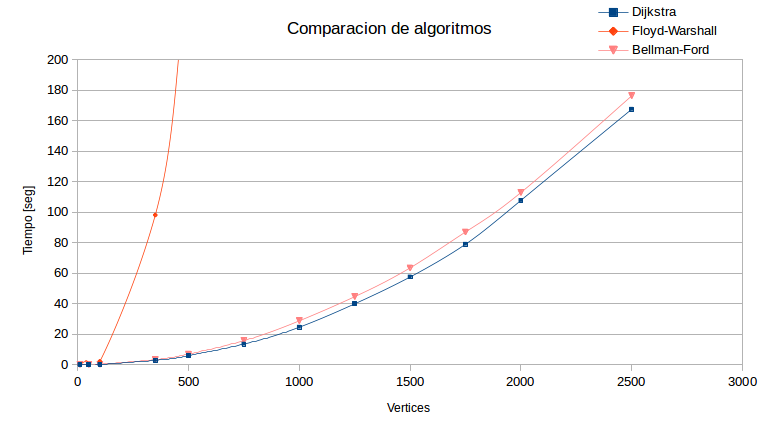
\includegraphics[width=9cm, height=5cm]{images/ComparacionAlgoritmos}
            \end{center}

        \subsection{Arbitrage}
            \tab Para resolver este problema lo que se puede hacer es cambiar los pesos de cada arista $W(E[u, v])$
            por un nuevo valor $W(E[u, v]) = -Log(W(E[u, v]))$ pues si nuestro objetivo es hallar un ciclo tal que
            $w_{1}*w_{2}*...*w_{k} > 1$ entonces buscamos un ciclo tal que $Log(w_{1}*w_{2}*...*w_{k}) > Log(1)$
            y por ende, queremos un ciclo tal que $-Log(w_{1}) - ... - Log(w_{k}) < 0$. Por lo tanto, si tenemos
            nuestros nuevos pesos, lo único que necesitamos es buscar ciclos negativos en nuestro grafo actualizado. \\
            \tab Para esto, como se mencionó en la sección anterior, se pueden utilizar tanto el algoritmo de
            Bellman-Ford como el de Floyd-Warshall.

        \subsection{Análisis individual de los algoritmos}

            \subsubsection{Dijkstra}
            \tab Como se mencionó previamente, el tiempo asintótico de este algoritmo es $O(|E|Log(|V|))$ y en la
            práctica los resultados son muy similares. \\
            \tab Aquí se muestra un gráfico del tiempo de ejecución en segundos, en función de la cantidad de vértices:
            \begin{center}
                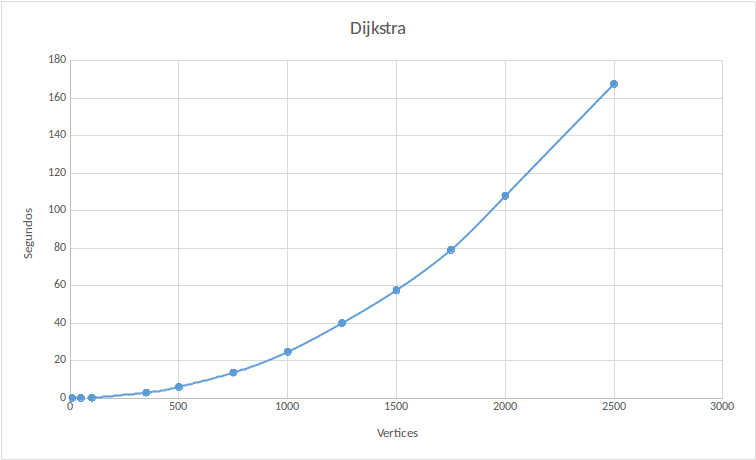
\includegraphics[width=9cm, height=5cm]{images/GraficoDijkstra}
            \end{center}
            \tab Y aquí se adjunta un gráfico en el que se compara, para los valores de $|V|$ de cada ejecución,
            la relación de la función $f(V, E) = |E|*Log(|V|)$ para el valor actual y el anterior, y la relación de
            tiempos de ejecución reales:
            \begin{center}
                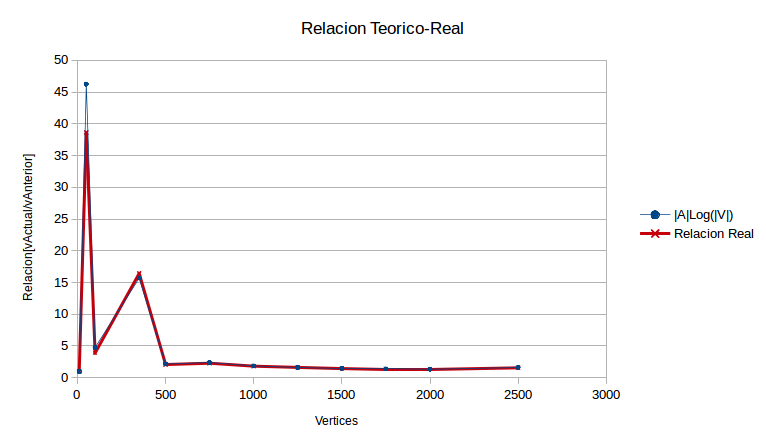
\includegraphics[width=9cm, height=5cm]{images/RelacionDijkstra}
            \end{center}
            \tab Este gráfico permite ver lo antes dicho: El tiempo de ejecución en la práctica es muy similar
            al teórico.

            \subsubsection{Floyd Warshall}
            \tab Como se mencióno en la sección 2.1.2, el tiempo asintótico de este algoritmo es $O(|V|^3)$ y en
            la práctica, al igual que Dijkstra, esta asíntota se respeta bastante. A raíz de esto, no fue posible
            ejecutar el algoritmo con muestras muy grandes ($|V| > 1000$) pero se obtuvieron muestras suficientes
            para obtener esta información de la relación tiempo de ejecución - cantidad de vértices:
            \begin{center}
                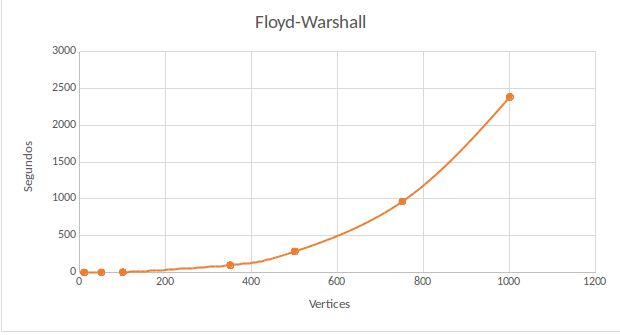
\includegraphics[width=9cm, height=5cm]{images/GraficoFloydWarshall}
            \end{center}
            \tab Y aquí se adjunta un gráfico en el que se compara, para los valores de $|V|$ de cada ejecución,
            la relación de la función $f(V, E) = |V|^3$ para el valor actual y el anterior, y la relación de
            tiempos de ejecución reales:
            \begin{center}
                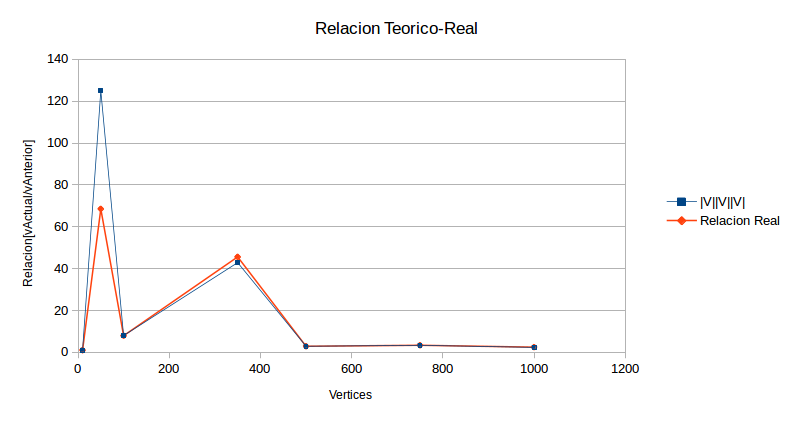
\includegraphics[width=9cm, height=5cm]{images/RelacionFloydWarshall}
            \end{center}
            \tab Este gráfico permite ver lo antes dicho: El tiempo de ejecución en la práctica es muy similar
            al teórico.

            \subsubsection{Bellman Ford}
            \tab Como antes se ha dicho, el tiempo asintótico de este algoritmo es $O(|V||E|)$, esto en el caso
            tratado en este trabajo se traduce a $O(|V|^3 - |V|^2)$. De todos modos, existe una optimización que,
            si bien no baja el tiempo asintótico, mejora mucho el tiempo promedio en la práctica. \\
            \tab Esta optimización se basa en, simplemente, verificar a cada paso de las $|V| - 1$ repeticiones
            si hubo alguna modificación en las distancias o padres de cada vértice y, en caso contrario, terminar
            la ejecución. De todos modos, cabe destacar que en caso de que haya ciclos negativos esta optimización
            no sirve de nada (pues siempre habrá un caso más optimo que el anterior). \\
            \tab Aquí se puede ver un gráfico comparativo de la ejecución del algoritmo optimizado y sin optimizar,
            en ambos casos sin ciclos negativos:
            \begin{center}
                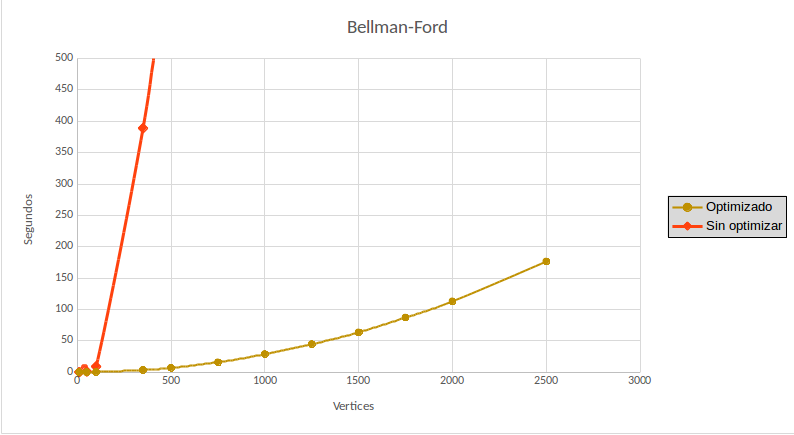
\includegraphics[width=9cm, height=5cm]{images/GraficoBellmanFord}
            \end{center}
            \tab Y aquí se adjunta un gráfico en el que se compara, para los valores de $|V|$ de cada ejecución,
            la relación de la función $f(V, E) = |V|*|E|$ para el valor actual y el anterior, y la relación de
            tiempos de ejecución reales:
            \begin{center}
                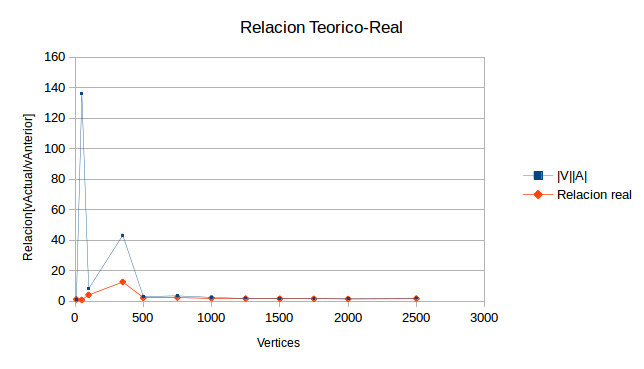
\includegraphics[width=9cm, height=5cm]{images/RelacionBellmanFord}
            \end{center}
            \tab En el gráfico de arriba se puede apreciar la optimización antes mencionada.

    \section{Comandos}


\end{document}
